\documentclass[usenames,xcolor={dvipsnames, table}]{beamer}
\usepackage[utf8]{inputenc}
\usepackage{lmodern}
\usepackage{verbatim}
\usetheme{uniud}
\usepackage{xparse}
\usepackage[spanish,es-tabla,es-nodecimaldot, es-nosectiondot, es-lcroman, es-noquoting]{babel}
\usepackage{subcaption}
\usepackage{array}
\usepackage{multirow}
\usepackage{multicol}
\usepackage{booktabs}
\usepackage{booktabs}
	\setlength\heavyrulewidth{0.9pt}

\usepackage{threeparttable}
\usepackage{amsmath}
\usepackage{nccmath}
\usepackage{etoolbox}
\usepackage{siunitx}

\makeatletter
\pretocmd\env@cases{\def\@rowc@lors{}}{}{}
\pretocmd\start@align{\def\@rowc@lors{}}{}{}
\makeatother

\newsavebox{\bmatrixbox}
\newenvironment{colorbmatrix}
  {\begin{lrbox}{\bmatrixbox}
   \mathsurround=0pt
   $\displaystyle
   \begin{bmatrix}}
  {\end{bmatrix}$%
   \end{lrbox}%
   \usebox{\bmatrixbox}%
   \kern-\wd\bmatrixbox
   \makebox[0pt][l]{$\left[\vphantom{\usebox{\bmatrixbox}}\right.$}%
   \kern\wd\bmatrixbox
}

% \ExplSyntaxOn
% \NewDocumentCommand{\convertto}{mm}
% % #1 = em or ex (or any other unit)
% % #2 = dimen to convert
% {
% 	\texttt{#2~=~\fp_to_decimal:n { (#2)/(1#1) }#1}
% }
% \ExplSyntaxOff

%%% Some useful commands
% pdf-friendly newline in links
\newcommand{\pdfnewline}{\texorpdfstring{\newline}{ }} 
% Fill the vertical space in a slide (to put text at the bottom)
\newcommand{\framefill}{\vskip0pt plus 1filll}


\title[Universidad Nacional Experimental del Tachira]{Laboratorio virtual de sistemas de control clasicos y difusos utilizando software libre}
\date[Marzo 2020]{Marzo 05, 2020}
\author[Proyecto Especial de Grado]{
  \textbf{Autor}: \hfill \\ Br. Kleiver J. Carrasco M. \\ \vspace{10pt} \textbf{Tutor}: \\ MSc. Ing. Juan R. Vizcaya R.
}

\institute{
	Universidad Nacional Experimental del Tachira

	Vicerrectorado Academico
	
	Decanato de Docencia
	
Departamento de Electronica
}

\begin{document}

\begin{frame}
	\titlepage
\end{frame}

\begin{frame}
	\frametitle{INTRODUCCIÓN}
	\vspace{20pt}

	\begin{block}{Planteamiento del problema}
		\begin{itemize}
			\large 
			\item ¿Es posible realizar un laboratorio para el análisis de sistemas de control con software libre?
			\item ¿Cumpliría con los requisitos para analizar, diseñar y simular sistemas de control?
			\item ¿Cómo se desempeñaría en comparación con otras herramientas?
		\end{itemize}
	\end{block}

	\begin{block}{¿Por qué ``Laboratorio Virtual''?}
		\begin{figure}
				\centering
				\begin{subfigure}[b]{0.2\linewidth}
					
\includegraphics[width=\linewidth]{imagenes/logoMATLAB}
				\end{subfigure}
				\hspace{0.8cm}
				\begin{subfigure}[b]{0.25\linewidth}
					
\includegraphics[width=\linewidth]{imagenes/logoSciLab}
				\end{subfigure}
				
			\end{figure}
	\end{block}
\end{frame}

\begin{frame}
	\frametitle{OBJETIVOS}
	\vspace{20pt}
	\begin{block}{Objetivo General}
		Desarrollar un laboratorio virtual de sistemas de control clásicos y difusos utilizando software libre.
	\end{block}
	
	\begin{block}{Objetivos específicos}
		\begin{enumerate} 
			\item Estudiar los sistemas de control clásicos.
			\item Estudiar el diseño de controladores difusos tipo Mamdani.
			\item Codificar las rutinas de análisis, diseño y simulación de sistemas de control necesarias.
			\item Realizar la interfaz gráfica de un laboratorio de sistemas de control virtual.
			\item Comparar los resultados obtenidos con dos herramientas de corte similar.
		\end{enumerate}
	\end{block}
	
\end{frame}

\begin{frame}
	\frametitle{METODOLOGIA}

	\vspace{20pt}
	
	\begin{block}{Tipo de investigación}
		Investigación proyectiva
	\end{block}

	\begin{block}{Modalidad}
		Proyecto factible
	\end{block}

	\begin{block}{Fases de la investigacion}
		\begin{itemize}
			\item Fase 1: Estudio de los sistemas de control clásicos y difusos
			\item Fase 2: Codificación de rutinas
			\item Fase 3: Interfaz gráfica y enlace con rutinas
			\item Fase 4: Comparación de resultados
		\end{itemize}
	\end{block}	
\end{frame}

\begin{frame}
	\frametitle{CONCEPTOS BASICOS}
	\vspace{20pt}

	\begin{itemize}
		\Large
		\setlength\itemsep{1em}
		\item Control de procesos
		\begin{itemize}
			\large
			\item[--] Control continuo
			\item[--] Control discreto
			\item[--] Control en lazo cerrado
			\item[--] Controlador PID
			\begin{block}{Ecuacion general en tiempo continuo de un controlador PID}
				\begin{equation}
					sc(t) = K_{p}e(t)+  K_{i}\int_{0}^{t} e(\tau) d\tau + K_{d} \frac{d}{dt}e(t)
				\end{equation}
			\end{block}
		\end{itemize}
		\item Métodos de Runge-Kutta
		\begin{itemize}
			\large
			\item[--] Métodos explícitos
			\item[--] Métodos embebidos
		\end{itemize} 
	\end{itemize}
	
\end{frame}

\begin{frame}
	\frametitle{CONCEPTOS BASICOS}
	\vspace{25pt}

	\begin{itemize}
		\Large
		\setlength\itemsep{1em}
		\item Lógica Difusa
		\begin{itemize}
			\large
			\setlength\itemsep{1em}
			\vspace{1em}
			\item[--] Controlador difuso
			\item[--] Controlador Mamdani 
		\end{itemize}
	\end{itemize}

	\begin{figure}
		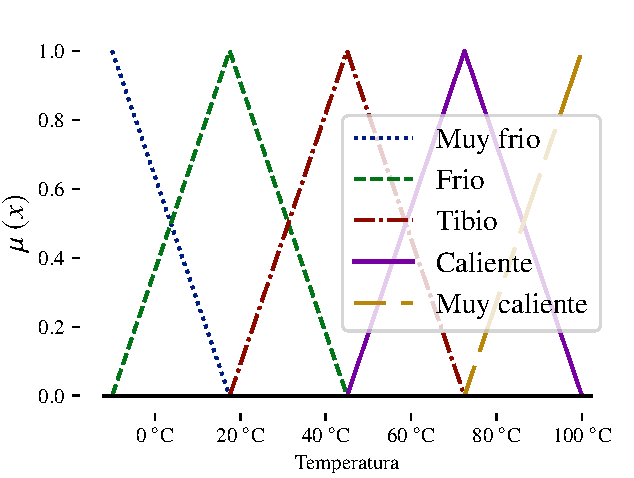
\includegraphics[width=0.5\linewidth]{imagenes/FuzzySet.pdf}
	\end{figure}
	\vspace{-20pt}
	\begin{itemize}
		\Large
		\item Python
	\end{itemize}

\end{frame}

\begin{frame}
	\frametitle{ESTRUCTURA DEL CODIGO: UML}
	\vspace{20pt}
	\begin{figure}
		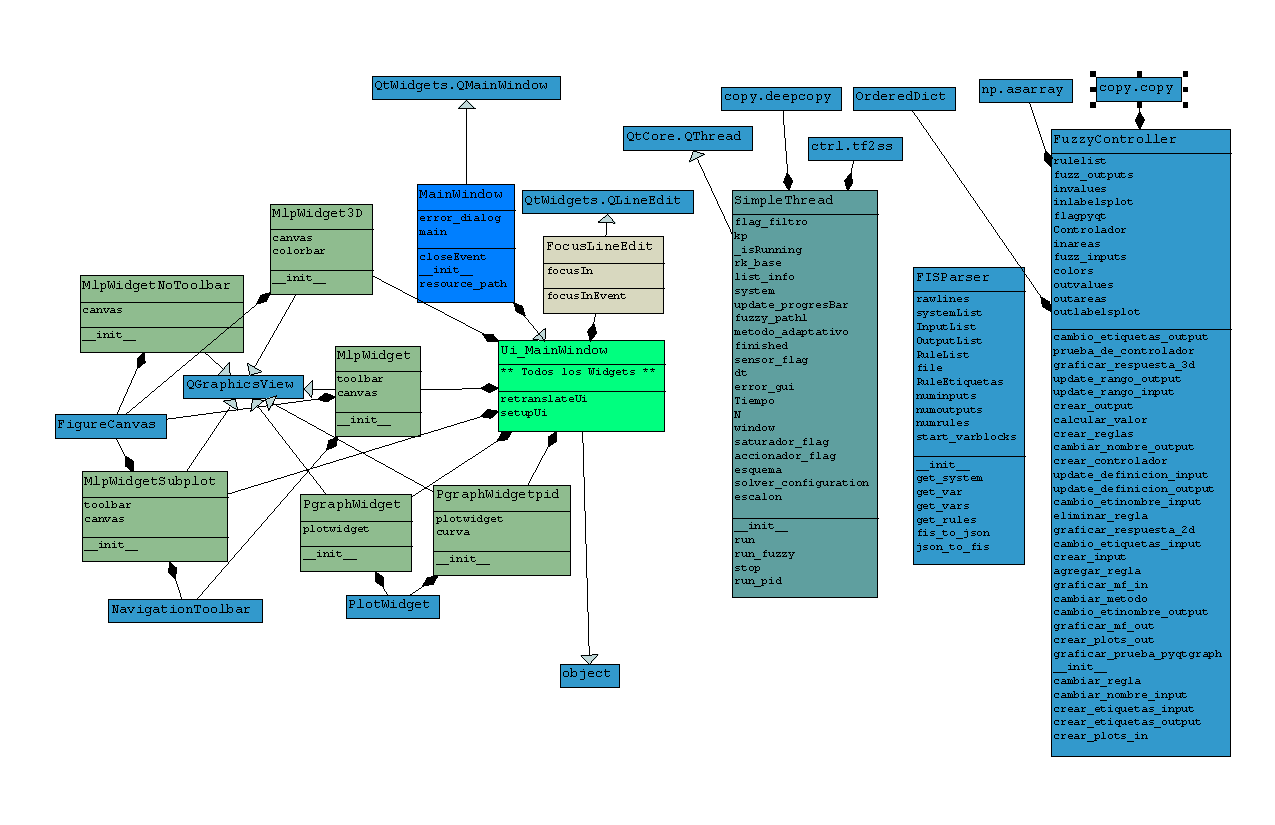
\includegraphics[width=\linewidth]{imagenes/UMLsinHandlers.pdf}
	\end{figure}
\end{frame}

\begin{frame}
	\frametitle{ESTRUCTURA DEL CODIGO: ESQUEMA}
	\vspace{20pt}
	\begin{figure}
		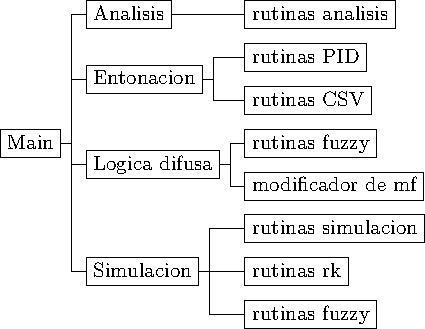
\includegraphics[width=0.9\linewidth]{imagenes/estructuraMain.pdf}
	\end{figure}
\end{frame}

\begin{frame}
	\frametitle{COMPARACION}
	\framesubtitle{ANALISIS}
	% \vspace{20pt}
	\rowcolors{1}{UniBlue!33}{UniBlue!7}
	{\centering
	\begin{table}[t]
		\centering 
		\hspace*{-0.6cm}
		\begin{threeparttable}
			% \setlength{\tabcolsep}{6pt}			% Separacion de columnas
			\setlength{\arraycolsep}{1pt}
			\scriptsize
			\renewcommand{\arraystretch}{3}
			\caption[Sistemas para la comparación de análisis de sistemas de control]{Sistemas para la comparación de análisis de sistemas de control}
			\begin{tabular*}{\textwidth}{c @{\extracolsep{\fill}}c}
					 {\normalsize Continuo} & {\normalsize Discreto} \\\renewcommand{\arraystretch}{3}
			$\dfrac{1}{s^2 + s + 1} $ & $\dfrac{0.004833 z+0.004675}{z^2 - 1.895 z + 0.9048} $  \\[5pt]
			\begin{tabular}[x]{cc} \setlength\arraycolsep{2pt} \renewcommand{\arraystretch}{1} $\begingroup \setlength\arraycolsep{2pt} A=\begin{colorbmatrix} -0.5 & -3 & -0.2 \\
				1 & 0 & 0 \\
				0 & 1 & 0 
			\end{colorbmatrix} \endgroup $ &  \renewcommand{\arraystretch}{1}
			$B=\begin{colorbmatrix} 1 \\ 0 \\ 0 \end{colorbmatrix}$ \\ \renewcommand{\arraystretch}{1}
			$C=\begin{colorbmatrix} 1 & 2 & 0.5 \end{colorbmatrix}$ & \renewcommand{\arraystretch}{1}
			$D=\begin{colorbmatrix} 0 \end{colorbmatrix}$ \end{tabular} & \begin{tabular}[x]{cc} \renewcommand{\arraystretch}{1} $A=\begin{colorbmatrix} 851.5 & -559.2 & -37.03 \\
				185.2 & 944.1 & -3.703 \\
				18.52 & 194.4 & 999.6 
			\end{colorbmatrix}_{10^{-3}} $ &  \renewcommand{\arraystretch}{1}
			$B=\begin{colorbmatrix} 185.2 \\ 18.52 \\ 1.852 \end{colorbmatrix}_{10^{-3}}$ \\ \renewcommand{\arraystretch}{1}
			$C=\begin{colorbmatrix} 1.116 & 1.713 & 0.4777 \end{colorbmatrix}$ & \renewcommand{\arraystretch}{1}
			$D=\begin{colorbmatrix} 0.1116 \end{colorbmatrix}$ \end{tabular} \\[15pt] 
			$\dfrac{s + 2}{s^2 + 0.5s + 3}e^{-1.5s} $ & $z^{-30}\left(\dfrac{0.02561 z^2 + 0.003084  z - 0.02375}{z^2 - 1.968 z + 0.9753}\right)$\\[8pt]
			\end{tabular*}
			\label{tab:AnalisisSistemas}
		\end{threeparttable}
	\end{table}}
\end{frame}

\begin{frame}
	\frametitle{COMPARACION}
	\framesubtitle{ANALISIS}
	\vspace{20pt}
	\small
	\begin{block}{Funciones de analisis}
		\footnotesize
		\begin{multicols}{2}
		\begin{itemize}
			\item Respuesta al escalón
			\item Respuesta al impulso
			\item Bode
			\item Nyquist
			\item Lugar de las raíces 
			\item Diagrama de Nichols
		\end{itemize}
	\end{multicols}
	\end{block}

	\begin{block}{Metricas empleadas}
		\footnotesize
		\begin{multicols}{2}
		\begin{itemize}
			\item Diferencia absoluta
			\item Diferencia porcentual
			\item Diferencia de área
			\item Raíz del error cuadrático medio (RECM)
			\item Distancia de energía
		\end{itemize}
	\end{multicols}
	\end{block}

	\rowcolors{1}{UniBlue!33}{UniBlue!7}
	\begin{table}
		\begin{tabular}{rcc}
										& Continuo 			& Discreto 			\\
		Diferencia absoluta promedio	& \num{8.980E-02}	& \num{1.057E-01}	\\
		RECM promedio					& \num{1.644E-02}	& \num{1.307E-02} 	\\
		\end{tabular}
	\end{table}
\end{frame}
\end{document}